\documentclass[10pt,twocolumn]{article}
\usepackage[T1]{fontenc}
\usepackage{lmodern,microtype}
\usepackage[letterpaper,margin=.72in,columnsep=.27in]{geometry}
\usepackage{amsmath,amssymb,amsthm,mathtools,enumitem,booktabs}
\usepackage{graphicx,tikz}
\usepackage{float}
\floatstyle{plain}
\newfloat{algorithm}{tbp}{loa}
\floatname{algorithm}{Algorithm}
\usepackage{pgfplots}
\pgfplotsset{compat=1.18}
\usetikzlibrary{arrows.meta,positioning,shapes.geometric}
\definecolor{cellblue}{RGB}{40,95,150}
\definecolor{cellorange}{RGB}{190,100,25}
\usepackage[hidelinks]{hyperref}
\setlength{\emergencystretch}{3em}
\newtheorem{theorem}{Theorem}[section]
\newtheorem{lemma}[theorem]{Lemma}
\newtheorem{proposition}[theorem]{Proposition}
\newtheorem{corollary}[theorem]{Corollary}
\theoremstyle{definition}\newtheorem{definition}{Definition}[section]
\theoremstyle{remark}\newtheorem{remark}[theorem]{Remark}
\newcommand{\R}{\mathbb R}\newcommand{\Q}{\mathbb Q}\newcommand{\Z}{\mathbb Z}
\newcommand{\eps}{\varepsilon}
\newcommand{\poly}{\operatorname{poly}}
\newcommand{\osc}{\operatorname{osc}}
\newcommand{\bits}{\operatorname{bits}}
\newcommand{\norm}[1]{\lVert#1\rVert}
\title{A Short Proof of a Range-Relative FPTAS\\for Polynomial Integer Optimization over Bounded Polyhedra}
\author{Robert Hildebrand\thanks{Developed with assistance from OpenAI's Codex assistant; see the disclosure at the end of the paper and the extended manuscript.}}
\date{}
\begin{document}\raggedbottom
\maketitle
\begin{abstract}
We give a short proof of a fully polynomial-time range-relative approximation scheme for polynomial optimization over the integer points of a bounded rational polyhedron in fixed dimension. Boundedness supplies a finite slack decomposition and a finite integer objective range. The proof combines the reflecting-set decomposition of Cook, Hartmann, Kannan, and McDiarmid with Markov's inequality and uses one integer linear feasibility query per refined cell. The running time is polynomial in the input encoding length, the numerical degree, and the reciprocal accuracy.
\end{abstract}

\section{Introduction and main result}

Let $P=\{\mathbf{x}\in\R^d:A\mathbf{x}\le\mathbf b\}$ be a bounded rational polyhedron, with $A\in\Q^{m\times d}$ and $\mathbf b\in\Q^m$, and let $f\in\Z[x_1,\ldots,x_d]$. We study
\begin{equation}\label{eq:problem}
 \begin{aligned}
 \min\quad & f(\mathbf{x})\\
 \text{s.t.}\quad & A\mathbf{x}\le\mathbf b,\\
 & \mathbf{x}\in\Z^d.
 \end{aligned}
\end{equation}
When $P\cap\Z^d\ne\varnothing$, choose minimizers and maximizers $\mathbf{x}_{\min},\mathbf{x}_{\max}$ and write $f_{\min}=f(\mathbf{x}_{\min})$ and $f_{\max}=f(\mathbf{x}_{\max})$.

De Loera, Hemmecke, K\"oppe, and Weismantel established an FPTAS for nonnegative polynomial maximization and a range-relative scheme for arbitrary polynomials in fixed dimension~\cite{DHKW06,DHKW08}. We give a short geometric proof for the bounded integer problem, using integer linear feasibility and an explicit bit-complexity bound. The guarantee is invariant under translation of the objective; it is not a multiplicative approximation to a nonnegative minimum.

The key ingredient is decomposition by relative constraint slacks. The reflecting sets of Cook, Hartmann, Kannan, and McDiarmid~\cite{CHKM} underpin their integer-hull analysis; related symmetric covers appear in the quadratic and cubic algorithms of Ari and Hildebrand~\cite{AHIQP,AH}, and dyadic slack grouping also appears in Wei's quadratic algorithm~\cite{Wei}. Here refinement produces long feasible integer progressions. Markov's inequality on these progressions controls the error at an integer optimum, allowing any feasible representative of its cell. The same representatives work for all polynomials of a prescribed degree.

\begin{figure*}[t]
\centering
{\small\bfseries Algorithm at a glance}\par\medskip
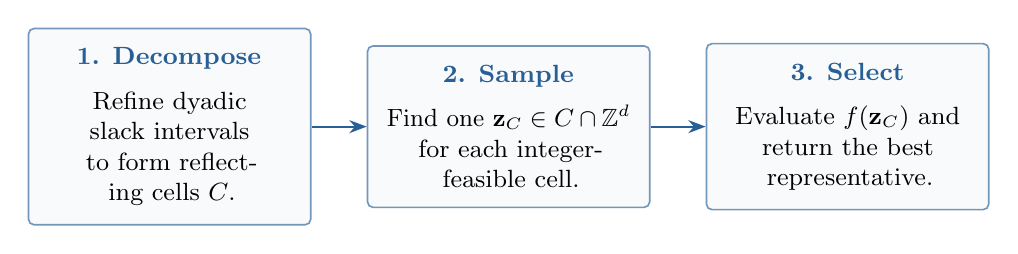
\begin{tikzpicture}[
  stage/.style={draw=cellblue!65,line width=.6pt,rounded corners=2pt,
    fill=cellblue!3,text width=.255\textwidth,minimum height=2.05cm,
    inner sep=7pt,align=center,font=\small},
  flow/.style={-{Stealth[length=2.2mm]},line width=.8pt,cellblue},
  node distance=7mm]
\node[stage] (decompose) {
  {\color{cellblue}\bfseries 1. Decompose}\\[5pt]
  Refine dyadic slack intervals\\
  to form reflecting cells $C$.
};
\node[stage,right=of decompose] (sample) {
  {\color{cellblue}\bfseries 2. Sample}\\[5pt]
  Find one $\mathbf z_C\in C\cap\Z^d$\\
  for each integer-feasible cell.
};
\node[stage,right=of sample] (select) {
  {\color{cellblue}\bfseries 3. Select}\\[5pt]
  Evaluate $f(\mathbf z_C)$ and\\
  return the best representative.
};
\draw[flow] (decompose)--(sample);
\draw[flow] (sample)--(select);
\end{tikzpicture}
\end{figure*}

The algorithm follows the decompose--sample--select procedure summarized in the overview. No local objective model is optimized. The proof separates the reflecting geometry (Section~\ref{sec:cover}) from enumeration and bit complexity (Section~\ref{sec:algorithm}).

To state the complexity bound precisely, we fix the following encoding convention. Vectors are columns and are written in bold. For an integer $u$, set $\langle u\rangle=1+\lceil\log_2(1+|u|)\rceil$. A rational number $u/v$ is stored in lowest terms with $v>0$, with size $\langle u/v\rangle=\langle u\rangle+\langle v\rangle$. For matrices, vectors, and lists, $\langle\cdot\rangle$ is the sum of the entry sizes together with the binary sizes of the dimensions and list lengths. The polynomial is supplied explicitly as
\[
 f(\mathbf{x})=\sum_{\alpha\in\mathcal A}c_\alpha\mathbf{x}^\alpha,
 \qquad c_\alpha\in\Z,\quad \alpha\in\Z_+^d,\quad |\alpha|_1\le D.
\]
Following~\cite{DHKW08}, coefficients are encoded in binary and exponent vectors in unary: each exponent $\alpha_j$ occupies $\alpha_j+1$ symbols. Thus $\langle f\rangle$ includes the coefficient sizes and $\sum_{\alpha\in\mathcal A}\sum_{j=1}^d(\alpha_j+1)$, together with dimensions and list lengths. Write $\varphi=\langle A,\mathbf b,f,\eps\rangle$ for the total input encoding size. We compute $D=\max\{1,\deg f\}$ from the nonzero monomials, taking $D=1$ for the zero polynomial; no separate degree input is needed. We retain $D$ explicitly in the running-time bound to show its contribution.

\begin{definition}[Range-relative FPTAS]\label{def:fptas}
Under the encoding convention above and for fixed dimension $d$, a range-relative fully polynomial-time approximation scheme is an algorithm that, for every rational $0<\eps\le1$, reports infeasibility when $P\cap\Z^d=\varnothing$, and otherwise returns $\mathbf{x}_{\eps}\in P\cap\Z^d$ satisfying
\begin{equation}\label{eq:guarantee}
 0\le f(\mathbf{x}_{\eps})-f_{\min}\le\eps(f_{\max}-f_{\min}).
\end{equation}
Its running time is polynomial in the total input encoding size $\varphi$ and $1/\eps$. The polynomial may depend on the fixed dimension. This is the fully polynomial-time weak-approximation notion of~\cite{DHKW08}. The maximization definition uses $f_{\max}-f(\mathbf{x}_{\eps})$ on the left.
\end{definition}

All complexity statements below count bit operations. The function $\poly$ denotes a polynomial with an absolute exponent, independent of $d,D,\eps$; different occurrences may denote different polynomials. Logs are base two unless indicated otherwise.

\begin{theorem}[Polynomial approximation by reflecting cells]\label{thm:main}
Let $d\ge1$ and let $P=\{\mathbf{x}\in\R^d:A\mathbf{x}\le\mathbf b\}$ be bounded, with $A\in\Z^{m\times d}$ and $\mathbf b\in\Z^m$, let $f\in\Z[x_1,\ldots,x_d]$, and put $D=\max\{1,\deg f\}$, with $D=1$ when $f=0$. For rational $0<\eps\le1$, let $\varphi=\langle A,\mathbf b,f,\eps\rangle$ be the total input encoding size.
There is a deterministic algorithm that reports infeasibility or returns $\mathbf{x}_{\eps}\in P\cap\Z^d$ satisfying~\eqref{eq:guarantee}, in at most
\begin{equation}\label{eq:runtime-coarse}
 \left(\frac{\varphi D}{\eps}\right)^{O(d)}
\end{equation}
bit operations, with an absolute constant in the $O(d)$ exponent.
\end{theorem}

Since the input explicitly lists the $m$ inequalities in $d$ variables, $m,d\le\varphi$; their separate factors in the detailed running-time bound are therefore absorbed into the base $\varphi$ and the $O(d)$ exponent in~\eqref{eq:runtime-coarse}. The dependence on dimension remains explicit in that exponent. More precisely, for fixed $P,D,d$, the algorithm makes $O(\eps^{-d/2})$ integer-feasibility queries; the detailed running-time bound in the proof retains the factor $\max\{D^2,D/\sqrt\eps\}$.

Rational inequalities can be normalized to integral data in polynomial time, as detailed below. Rational objective coefficients can likewise be reduced to integer coefficients by clearing denominators in polynomial time; positive scaling preserves the approximation guarantee, as in~\cite[Section~5]{DHKW08}. The remaining construction parameters and the exact feasibility-query count are introduced in the proof. For fixed $d$, the bound is polynomial in $\varphi$ and $1/\eps$, hence gives an FPTAS in Definition~\ref{def:fptas}. The same explicit bound remains valid for binary-encoded exponents, but then its numerical dependence on $D$ does not assert an FPTAS in the sparse binary input size.

\begin{corollary}[Nonnegative maximization]\label{cor:max}
Under the same assumptions and encoding conventions, if $f\ge0$ on $P\cap\Z^d$, choosing the largest objective value among the representatives yields
\[
 f(\mathbf{x}_{\eps})\ge(1-\eps)f_{\max}.
\]
Thus the construction gives a multiplicative FPTAS for nonnegative maximization under the encoding convention of Definition~\ref{def:fptas}.
\end{corollary}

\begin{corollary}[Mixed-integer approximation]\label{cor:mixed}
Fix the total dimension $d=d_c+d_i$. Let $P=\{\mathbf{x}\in\R^d:A\mathbf{x}\le\mathbf b\}$ be a bounded rational polyhedron and $f\in\Z[x_1,\ldots,x_d]$. Under the same encoding convention, for rational $0<\eps\le1$ there is an algorithm, polynomial in $\varphi=\langle A,\mathbf b,f,\eps\rangle$ and $1/\eps$, that reports infeasibility or returns
\[
\begin{gathered}\mathbf{x}_{\eps}\in P\cap(\Q^{d_c}\times\Z^{d_i}),\\
 0\le f(\mathbf{x}_{\eps})-f_{\min}\le\eps(f_{\max}-f_{\min}),
\end{gathered}\]
where the extrema are over $P\cap(\R^{d_c}\times\Z^{d_i})$. For nonnegative $f$ on this set, a multiplicative FPTAS for maximization is obtained as well.
\end{corollary}

Corollary~\ref{cor:mixed} combines our integer algorithm with the grid reduction of De Loera et al.~\cite{DHKW08}; it does not require a reflecting-cell cover of the entire mixed-integer feasible set.

\paragraph{Comparison with prior algorithms.}

The generating-function approach of De Loera et al.~\cite{DHKW06,DHKW08} computes weighted sums involving $f^q$, where $q=O(1+\eps^{-1}\log N)$ and $N=|P\cap\Z^d|$. The standard Barvinok counting bound is $\langle A,\mathbf b\rangle^{O(d\log(d+1))}$~\cite[Theorem~2.3]{PakPanova}; our entire algorithm has bound $\varphi^{O(d)}$ for fixed $D,\eps$. This compares available upper bounds, not a runtime separation: counting alone does not describe their FPTAS, and our potentially large cell count does not establish practical superiority.

Del Pia's quadratic scheme~\cite[Proposition~3 and Section~6.2]{DelPia} uses affine optimization over boxes after geometric preprocessing, with flatness recursion in the remaining cases. For fixed quadratic rank $k$ and integer dimension $p$, it uses $O_{k,p}(1+\eps^{-k/2})$ MILP subproblems and allows variable continuous dimension. Our feasibility-call exponent matches $k/2$ at $k=d$, but our enumeration costs an additional factor of order $\eps^{-1/2}$. Our advantages are arbitrary degree and objective-independent representatives; we do not recover his low-rank dependence.

\section{Reflecting cells and approximation}\label{sec:cover}

We first construct cells supporting feasible integer progressions, then apply Markov's inequality along a progression through an integer optimum. Neither the optimum nor the objective range is needed by the algorithm.

Clear rational row denominators by multiplying each row by the product of its positive denominators. This takes polynomial time; normalized entries have $O(\varphi)$ bits. Equalities may be represented by pairs of inequalities, and lower-dimensional polytopes are allowed. Real feasibility and boundedness are testable by rational linear programming; boundedness remains a hypothesis of our theorem.

For the remainder of the construction, $A,\mathbf b$ denote the normalized integral data; $\varphi$ continues to denote the original input size. To track the construction explicitly, define
\begin{equation}\label{eq:tau}
 \tau=\left\lceil\log_2\bigl(2+\max\{\|A\|_{\max},\|\mathbf b\|_\infty\}\bigr)\right\rceil.
\end{equation}
Here $\|A\|_{\max}$ is the largest absolute matrix entry, so $\tau$ measures coefficient size rather than magnitude. The remaining parameters have the following roles: $V$ bounds coordinate lengths, $M$ is the number of dyadic slack scales, $\ell$ is the refinement, and $H$ bounds the number of hyperplanes. Set
\begin{align}
 V&=d\bigl(\tau+\lceil\log_2(d+1)\rceil\bigr)+2,\label{eq:V}\\
 M&=\tau+V+\lceil\log_2(d+1)\rceil+2,\label{eq:M}\\
 \ell&=\max\{D^2,\lceil D/\sqrt\eps\rceil\},\qquad H=m(M\ell+2),\label{eq:HT}\\
 F_d(H)&=\sum_{j=0}^{d}2^j\binom Hj\le(1+2H)^d.\label{eq:F}
\end{align}

\begin{lemma}[Coordinates and slacks]\label{lem:size}
If $P\ne\varnothing$, every $\mathbf{x}\in P$ satisfies $|x_j|<2^V$ for every $j$. Every slack $s_i(\mathbf{x})=b_i-\mathbf{a}_i^\top \mathbf{x}$ satisfies $0\le s_i(\mathbf{x})<2^M$, with $V,M$ defined in~\eqref{eq:V}--\eqref{eq:M}.
\end{lemma}
\begin{proof}
A vertex of a bounded polyhedron in $\R^d$ has $d$ linearly independent active constraint normals, including when the polyhedron is lower-dimensional. Cramer's rule expresses each vertex coordinate as a ratio of two integral determinants of order $d$. The nonzero denominator has absolute value at least one. Since every entry of $A,\mathbf{b}$ has absolute value less than $2^\tau$, the absolute value of a numerator is at most $d!2^{d\tau}\le d^d2^{d\tau}<2^V$. Every point of $P$ is a convex combination of vertices. Finally,
\[
 s_i(\mathbf{x})\le |b_i|+\sum_{j=1}^d|a_{ij}|\,|x_j|
 <2^\tau(1+d2^V)<2^M.
\]
\end{proof}

The preceding bounds identify a finite interval of relevant slack values. At an integer point, each slack is either zero or at least one. This gap allows us to cover all positive integer slacks using finitely many dyadic scales, even when the polytope is thin or lower-dimensional. Within each scale, the refinement controls relative slack variation; this is what permits extrapolation beyond the cell.

The dyadic construction in~\cite[Theorem~2.2]{AH}, tracing back to~\cite{CHKM}, groups comparable positive slacks. We retain their notation $s_i$, $C$, and $D_C$ for slacks, cells, and symmetric displacement sets. Figure~\ref{fig:pentagon-cells} illustrates the construction on a pentagon. Our refinement parameter $\ell\ge1$ strengthens $C-C\subseteq D_C$ to $\ell(C-C)\subseteq D_C$.

\begin{definition}[Refined thresholds]\label{def:thresholds}
For integers $M,\ell\ge1$, let
\begin{equation}\label{eq:thresholds}
\begin{split}\mathcal B_{M,\ell}=\{0,2^M\}\cup\\
 \left\{2^k\left(1+\frac{j}{\ell}\right):0\le k<M,\ 0\le j<\ell\right\}
.\end{split}
\end{equation}
There are $M\ell+2$ thresholds. Insert the hyperplanes $s_i(\mathbf{x})=a$ for every row $i$ and every $a\in\mathcal B_{M,\ell}$, ignoring expressions that do not define proper hyperplanes. A cell is a nonempty relatively open face of this arrangement that lies in $P$. Discard cells having any slack in $(0,1)$.
\end{definition}

Including all faces is essential: integer points may lie on many threshold hyperplanes. Denote the retained cell family by $\mathcal C$. These cells cover $P\cap\Z^d$, because all slacks at integer points are nonnegative integers. Threshold zero ensures that an arrangement face cannot cross the boundary of $P$.

If $a<b$ are successive positive thresholds, then
\begin{equation}\label{eq:width}
 b-a\le a/\ell.
\end{equation}
Indeed, on a dyadic interval $[2^k,2^{k+1}]$ the spacing is $2^k/\ell$ and $a\ge2^k$. This includes its last subinterval. For $\ell=1$ the positive thresholds are exactly dyadic.

\begin{figure*}[t]
\centering
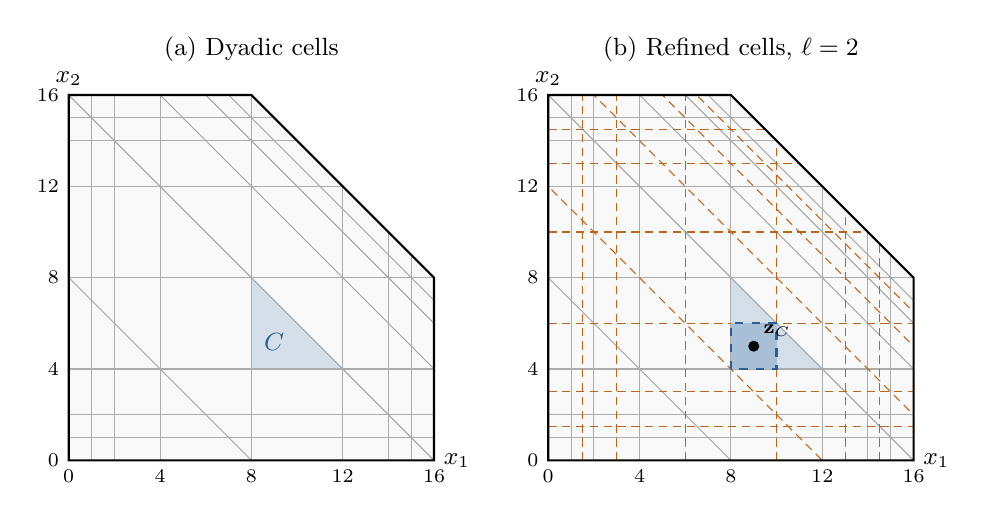
\begin{tikzpicture}[x=.29cm,y=.29cm,font=\small]
\foreach \shift/\panel/\refined in {0/{(a) Dyadic cells}/0,21/{(b) Refined cells, $\ell=2$}/1} {
  \begin{scope}[xshift=\shift*.29cm]
    \begin{scope}
      \clip (0,0)--(16,0)--(16,8)--(8,16)--(0,16)--cycle;
      \fill[gray!5] (0,0) rectangle (16,16);
      \fill[cellblue!20] (8,4)--(12,4)--(8,8)--cycle;
      \foreach \u in {1,2,4,8,12,14,15} {
        \draw[gray!65,thin] (\u,0)--(\u,16);
        \draw[gray!65,thin] (0,\u)--(16,\u);
      }
      % Fifth slack: 24-x_1-x_2. Each threshold gives a diagonal.
      \foreach \a in {1,2,4,8,16} {
        \draw[gray!65,thin] (-8,{32-\a})--(32,{-8-\a});
      }
      \ifnum\refined=1
        \foreach \u in {1.5,3,6,10,13,14.5} {
          \draw[cellorange,densely dashed,thin] (\u,0)--(\u,16);
          \draw[cellorange,densely dashed,thin] (0,\u)--(16,\u);
        }
        \foreach \a in {1.5,3,6,12,24} {
          \draw[cellorange,densely dashed,thin] (-8,{32-\a})--(32,{-8-\a});
        }
        \fill[cellblue!40] (8,4) rectangle (10,6);
        \draw[cellblue,thick,dashed] (8,4) rectangle (10,6);
        \fill (9,5) circle (2pt);
        \node[above right,font=\scriptsize] at (9,5) {$\mathbf z_C$};
      \else
        \node[cellblue] at (9,5.2) {$C$};
      \fi
    \end{scope}
    \draw[thick] (0,0)--(16,0)--(16,8)--(8,16)--(0,16)--cycle;
    \foreach \u in {0,4,8,12,16} {
      \node[below,font=\scriptsize] at (\u,0) {$\u$};
      \node[left,font=\scriptsize] at (0,\u) {$\u$};
    }
    \node at (8,18) {\panel};
    \node[right] at (16,0) {$x_1$};
    \node[above] at (0,16) {$x_2$};
  \end{scope}
}
\end{tikzpicture}
\caption{The slack-cell construction on the pentagon $P=\{\mathbf{x}\in[0,16]^2:x_1+x_2\le24\}$. The fifth slack, $24-x_1-x_2$, adds diagonal threshold lines, so cells need not be boxes. The shaded dyadic cell is the open triangle $x_1>8$, $x_2>4$, $x_1+x_2<16$. Refinement with $\ell=2$ introduces the dashed orange lines; the darker cell $(8,10)\times(4,6)$ contains the integer representative $(9,5)$. Both panels show the full arrangement before discarding open strips with slack in $(0,1)$; lower-dimensional faces are also cells.}
\label{fig:pentagon-cells}
\end{figure*}

\begin{lemma}[Refined displacement cover]\label{lem:reflection}
For each $C\in\mathcal C$, define
\[
 D_C=\{\mathbf{d}\in\R^d:|\mathbf{a}_i^\top\mathbf{d}|\le w_i\ (1\le i\le m)\},
\]
where $w_i=0$ for a slack constant on $C$, and $w_i=a$ for a slack in a positive interval $(a,b)$. Then
\[
 \ell(C-C)\subseteq D_C,\qquad C\pm D_C\subseteq P.
\]
In particular, for $\mathbf{x},\mathbf{y}\in C$,
\begin{equation}\label{eq:long}
 \mathbf{x}+t(\mathbf{y}-\mathbf{x})\in P\qquad(|t|\le\ell).
\end{equation}
\end{lemma}
\begin{proof}
Since cells with a slack in $(0,1)$ were discarded, every varying slack on a retained cell lies between successive thresholds $a<b$ with $a\ge1$. Thus the relative-width bound~\eqref{eq:width} applies.

For a varying slack, $|s_i(\mathbf{y})-s_i(\mathbf{x})|<b-a\le a/\ell$ and $s_i(\mathbf{x})>a=w_i$; for a constant slack the difference is zero. These inequalities give both inclusions row by row. The set $D_C$ is convex, symmetric, and contains zero, so it contains $t(\mathbf{y}-\mathbf{x})$ for $|t|\le\ell$. Also $D_C\subseteq P-\mathbf{x}$ for any $\mathbf{x}\in C$, hence it is bounded, as required for a symmetric displacement cover in~\cite[Definition~2.1]{AH}.
\end{proof}

\begin{remark}[Relative slacks characterize extrapolation]\label{rem:slack-characterization}
Let $\mathbf{x},\mathbf y\in P$, set $\mathbf v=\mathbf y-\mathbf{x}$, and let $\ell>0$. The segments $\mathbf{x}+[-\ell,\ell]\mathbf v$ and $\mathbf y+[-\ell,\ell]\mathbf v$, centered at $\mathbf{x}$ and $\mathbf y$ respectively, both lie in $P$ if and only if, for every row $i$,
\[
 \ell\,|s_i(\mathbf y)-s_i(\mathbf{x})|
 \le\min\{s_i(\mathbf{x}),s_i(\mathbf y)\}.
\]
Indeed, the minimum slack along the first segment is $s_i(\mathbf{x})-\ell|s_i(\mathbf y)-s_i(\mathbf{x})|$, and similarly for the second. For positive slacks the condition is equivalently
\[
 \frac{\max\{s_i(\mathbf{x}),s_i(\mathbf y)\}}
 {\min\{s_i(\mathbf{x}),s_i(\mathbf y)\}}\le1+\frac1\ell;
\]
if either slack is zero, both must be zero. Thus multiplicative slack control is exactly the geometry needed for extrapolation about both points. Refined dyadic intervals enforce this condition with short rational descriptions, and integrality limits the number of relevant scales. The condition is independent of the objective: Proposition~\ref{prop:extrema} turns the resulting cover into a simultaneous approximation guarantee for every polynomial of degree at most $D$.
\end{remark}

The displacement property is the only geometric input to the approximation argument. To obtain an algorithm, we also need a short list of cells and a linear description suitable for integer feasibility. Including every face of the arrangement handles points on threshold hyperplanes; rounding strict slack bounds then preserves exactly the integer points in each face.

\begin{lemma}[Number, encoding, and enumeration of cells]\label{lem:arrangement}
Let $H=m(M\ell+2)$ and set
\[
 B=\tau+M+\lceil\log_2(\ell+1)\rceil+10.
\]
There are at most $F_d(H)$ retained cells. Each cell has a description by at most two slack bounds per row, allowing equality or strict inequalities, with coefficient bit length $O(B)$. The cells can be enumerated deterministically in
\begin{equation}\label{eq:arrangement-time}
 (H+1)F_d(H)\,\poly(\langle A,\mathbf b\rangle+d+m+B)
\end{equation}
bit operations. Each cell can be converted to a closed rational polyhedron $\widehat C\subseteq C$ having exactly the same integer points, with at most $2m$ inequalities of bit length $O(\tau+M+1)$ per coefficient.
\end{lemma}
\begin{proof}
The total face count follows by induction on the number of hyperplanes. Inserting a new hyperplane replaces each relatively open face that it crosses by two side faces and their intersection, increasing the count by two. The crossed faces give distinct faces of the induced arrangement on the new hyperplane, which has dimension $d-1$ and at most $H-1$ hyperplanes. Faces contained in the new hyperplane are unchanged. Thus the maximum total face count satisfies
\[
\begin{gathered}T_d(H)\le T_d(H-1)+2T_{d-1}(H-1),\\
 T_d(0)=T_0(H)=1.\end{gathered}
\]
Pascal's identity shows that $F_d(H)=\sum_{j=0}^d2^j\binom Hj$ satisfies the corresponding equality, proving the bound. Restricting to retained cells cannot increase the count, and $F_d(H)\le(1+2H)^d$ gives~\eqref{eq:F}. See~\cite{Stanley} for general background on arrangements.

Every threshold in~\eqref{eq:thresholds} has a representation $N/\ell$, where $N=2^k(\ell+j)$ or the corresponding numerator for an endpoint. The numerator has $O(M+\log(\ell+1))$ bits and the denominator has $O(\log(\ell+1))$ bits. Multiplying a threshold equation by $\ell$ gives coefficients of bit length $O(B)$. Unlike repeated multiplication of $1+1/\ell$, this construction has no factor $\ell$ in the threshold bit length.

For completeness, an elementary incremental enumerator suffices. Start with $P$ and insert the threshold hyperplanes one at a time. For each retained sign region, test its intersections with the positive, zero, and negative side of the new hyperplane. Keep the nonempty regions. At each stage every region is the intersection of $P$ with an arrangement face; it has a unique sign vector, and there are at most $F_d(H)$ such regions. Constraints arising from the same original row can always be compressed to its strongest lower and upper slack bounds, recording whether a bound is strict. Equality is represented by equal bounds. Thus each feasibility test has $O(m)$ constraints, rather than $O(H)$ constraints.

To test real feasibility with strict inequalities, write each strict inequality as $u_j^\top \mathbf{x}<v_j$, introduce a common variable $\delta$, replace it by $u_j^\top \mathbf{x}\le v_j-\delta$, impose $0\le\delta\le1$, and maximize $\delta$. Keep the weak constraints and equalities unchanged. Feasibility of the strict system is equivalent to a positive optimal value; when there are no strict inequalities, use ordinary feasibility. This is an exact rational LP in at most $d+1$ variables. There are $O((H+1)F_d(H))$ tests. Comparisons and storage of the compressed descriptions satisfy the same bound. At termination discard any cell meeting the forbidden slack interval $(0,1)$.

Finally, the slack $s_i(\mathbf{x})$ is integral for integer $\mathbf{x}$. Replace $s_i(\mathbf{x})>a$ by $s_i(\mathbf{x})\ge\lfloor a\rfloor+1$, and replace $s_i(\mathbf{x})<b$ by $s_i(\mathbf{x})\le\lceil b\rceil-1$. If a slack is fixed at a nonintegral threshold, discard the cell as integer-infeasible; otherwise keep its integral equality. These replacements define a closed subset of the original cell with the same integer points. A slack constant at a nonintegral value that is not a threshold also leaves the cell integer-infeasible; the integer-feasibility query detects this case. Their right-hand sides have $O(\tau+M+1)$ bits, and their normals are rows of $A$ or their negatives. Equality may be stored as two inequalities. All arithmetic, including floor and ceiling, is exact.
\end{proof}

\begin{remark}[Parallel families]
If row $i$ contributes $q_i$ distinct threshold hyperplanes, the count can be sharpened to
\[
 |\mathcal C|\le
 \sum_{\substack{I\subseteq\{1,\ldots,m\}\\|I|\le d}}
 2^{|I|}\prod_{i\in I}q_i
 \le\sum_{j=0}^d2^j\binom mj(M\ell+2)^j.
\]
The insertion argument counts intersections involving at most one hyperplane from each parallel family; further dependencies can only reduce the count. This improves the bound without changing its worst-case $\ell^d$ dependence. We retain $F_d(H)$ for simplicity. The boundary-vertex count in~\cite[pp.~30--31]{CHKM} bounds integer-hull vertices, not all reflecting cells, and therefore does not directly replace this count.
\end{remark}

We next combine the sample-to-supremum argument used in polynomial norming meshes~\cite[Section~2]{PV} with a second-difference bound at a discrete minimum. Long progressions control variation between integer samples without assuming continuous stationarity.

\begin{lemma}[Approximation at a discrete minimum]\label{lem:markov}
Let $D\ge1$ and $\ell\ge D^2$ be integers, and let $p\in\R[t]$ have degree at most $D$. Suppose
\[
 a\le p(k)\le b\quad(k=-\ell,\ldots,\ell),\qquad p(-1)\ge p(0).
\]
Then
\[
 p(1)-p(0)\le \frac{D^2}{\ell^2}(b-a).
\]
\end{lemma}
\begin{proof}
Set $q=p-(a+b)/2$ and $W=\|q\|_{\infty,[-\ell,\ell]}$. The scaled classical Markov inequality gives $\|q'\|_\infty\le D^2W/\ell$; see~\cite[Theorem~1.1]{Pierzchala}. Every point of $[-\ell,\ell]$ lies within $1/2$ of a sampled integer, so
\[
 W\le \frac{b-a}{2}+\frac{D^2}{2\ell}W\le\frac{b-a+W}{2},
 \qquad W\le b-a.
\]
Let $n=\lfloor D/2\rfloor$. The even part of $q$ has the form
\[
 e(t)=\frac{q(t)+q(-t)}2=h(t^2),\qquad \deg h\le n.
\]
Thus $\|h\|_{\infty,[0,\ell^2]}\le W$. Markov's inequality on $[0,\ell^2]$ gives $\|h'\|_\infty\le 2n^2W/\ell^2$. Since $\ell\ge1$, the mean value bound on $[0,1]$ and $p(-1)\ge p(0)$ yield
\[
\begin{aligned}
 p(1)-p(0)&\le p(1)+p(-1)-2p(0)\\
 &=2(h(1)-h(0))\\
 &\le\frac{4\lfloor D/2\rfloor^2}{\ell^2}(b-a)
 \le\frac{D^2}{\ell^2}(b-a).
\end{aligned}
\]
For $D=1$, $h$ is constant and the bound is zero. The argument also covers $a=b$.
\end{proof}

The estimate is needed only on the cell containing a global minimizer, and holds for any representative of that cell. Applying it also to $-f$ gives the following simultaneous approximation of both extrema. This passage from sampling to optimization is standard; compare~\cite[Proposition~1]{PV}. The reflecting geometry supplies the feasible integer samples needed here.

\begin{proposition}[Representatives approximate extrema]\label{prop:extrema}
Choose one integer representative from each integer-feasible retained cell, forming $Y$. If $P\cap\Z^d\ne\varnothing$ and $\ell\ge D^2$, then every real polynomial $f$ of degree at most $D$ satisfies
\[
\begin{aligned}
 0&\le\min_Y f-\min_{P\cap\Z^d} f\le\frac{D^2}{\ell^2}(f_{\max}-f_{\min}),\\
 0&\le\max_{P\cap\Z^d} f-\max_Y f\le\frac{D^2}{\ell^2}(f_{\max}-f_{\min}).
\end{aligned}
\]
\end{proposition}
\begin{proof}
Let $\mathbf{x}_{\min}$ minimize $f$ on $P\cap\Z^d$, and let $\mathbf{y}$ represent its cell. Put $p(t)=f(\mathbf{x}_{\min}+t(\mathbf{y}-\mathbf{x}_{\min}))$. Lemma~\ref{lem:reflection} makes all integer samples with $|k|\le \ell$ feasible, so they lie between $f_{\min}$ and $f_{\max}$. Minimality gives $p(-1)\ge p(0)$. Lemma~\ref{lem:markov} now bounds $f(\mathbf{y})-f(\mathbf{x}_{\min})$. Apply the same argument to $-f$ for the maximum.
\end{proof}



\section{Algorithm and complexity}\label{sec:algorithm}

Algorithm~\ref{alg:sampling} enumerates the refined cells and compares their representatives. It accepts any degree bound $D\ge\max\{1,\deg f\}$; Theorem~\ref{thm:main} computes this bound from $f$. A constant objective requires only one integer feasibility query, and dimension zero is immediate. Representatives may be processed as a stream or saved for reuse.

\begin{algorithm}[tbp]
\centering
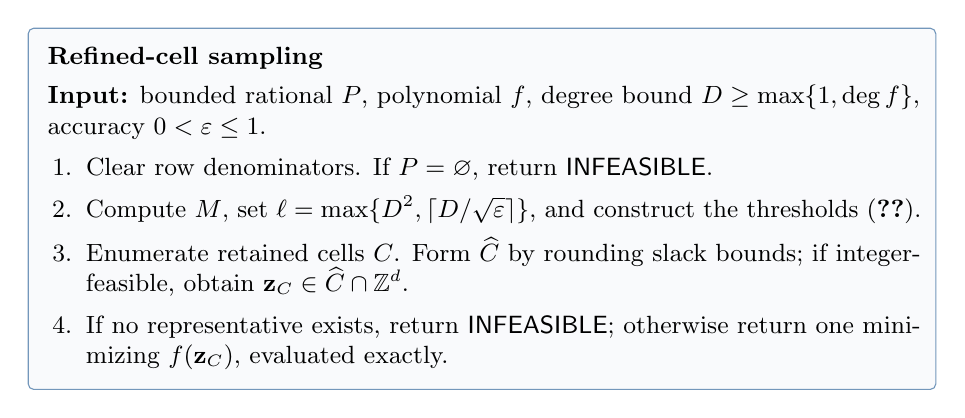
\begin{tikzpicture}
\node[draw=cellblue!65,rounded corners=2pt,fill=cellblue!3,inner sep=7pt] {
\begin{minipage}{.91\columnwidth}\small
\textbf{Refined-cell sampling}\par\smallskip
\textbf{Input:} bounded rational $P$, polynomial $f$, degree bound $D\ge\max\{1,\deg f\}$, accuracy $0<\eps\le1$.
\begin{enumerate}[leftmargin=1.5em,itemsep=2pt,topsep=4pt]
\item Clear row denominators. If $P=\varnothing$, return \textsf{INFEASIBLE}.
\item Compute $M$, set $\ell=\max\{D^2,\lceil D/\sqrt\eps\rceil\}$, and construct the thresholds~\eqref{eq:thresholds}.
\item Enumerate retained cells $C$. Form $\widehat C$ by rounding slack bounds; if integer-feasible, obtain $\mathbf z_C\in\widehat C\cap\Z^d$.
\item If no representative exists, return \textsf{INFEASIBLE}; otherwise return one minimizing $f(\mathbf z_C)$, evaluated exactly.
\end{enumerate}
\end{minipage}};
\end{tikzpicture}
\caption{The cover and representatives depend only on $P,D,\eps$.}
\label{alg:sampling}
\end{algorithm}

\begin{proof}[Correctness in Theorem~\ref{thm:main}]
Every integer-feasible cell contributes a feasible representative, and the retained cells cover $P\cap\Z^d$. Thus $Y=\varnothing$ if and only if $P\cap\Z^d=\varnothing$. Otherwise, Proposition~\ref{prop:extrema} and $\ell=\max\{D^2,\lceil D/\sqrt\eps\rceil\}$ give
\[
 0\le\min_Y f-f_{\min}\le \frac{D^2}{\ell^2}(f_{\max}-f_{\min})\le\eps (f_{\max}-f_{\min}).
\]
The algorithm returns a minimizer on $Y$. The cover and representatives depend only on $P,D,\eps$, so the same set works for every polynomial of degree at most $D$.
\end{proof}

It remains to account for bit operations. There are three costs: constructing the arrangement, producing integer representatives, and evaluating the objective. The distinction between the number of cells and the sizes of their descriptions is important: refinement increases the former polynomially in $1/\sqrt\eps$, whereas it increases the threshold bit lengths only logarithmically.
By Lemma~\ref{lem:arrangement}, face enumeration costs~\eqref{eq:arrangement-time}. The bit length of $\ell$ is $O(\log(D+1)+\langle\eps\rangle)$; compute the least positive integer $k$ satisfying $\eps k^2\ge D^2$ by binary search with rational comparisons, and set $\ell=\max\{D^2,k\}$. Generating all thresholds uses $O(M\ell)$ arithmetic operations on integers with $O(M+\log(\ell+1))$ bits and is included in the arrangement bound when $m\ge1$. A nonempty bounded polyhedron in positive dimension cannot be specified by zero inequalities.

Once a cell has been enumerated, its integer feasibility query has a description whose coefficient sizes do not grow with the refinement parameter.
Each of at most $F_d(H)$ queries has $d$ integer variables and a total encoding length
\begin{equation}\label{eq:ilp-size}
 S_C=O\!\left(m(d+1)(\tau+M+1)+d+m\right).
\end{equation}
Fixed-dimensional integer linear feasibility with witness production takes $2^{O(d\log(d+1))}S_C^{O(1)}$ bit operations using Kannan's algorithm~\cite{Kannan}, improving the dimension dependence of Lenstra's algorithm~\cite{Lenstra}. The feasibility query is made on a subset of the original bounded polytope. Accordingly, every returned coordinate has at most $V+O(1)$ bits by Lemma~\ref{lem:size}; its length is not proportional to its magnitude. Notice also that~\eqref{eq:ilp-size} has no dependence on $\ell$ other than the number of cells, because the threshold inequalities have already been rounded to integer slack bounds.

Finally, the coordinate bound ensures that exact objective evaluation also has polynomial bit cost, even though feasible coordinates can be numerically large.
The integer coefficients of $f$ have bit length at most $\langle f\rangle$. If $\mathbf{x}\in P\cap\Z^d$, every monomial has absolute value at most $2^{DV}$. Each value of $f(\mathbf{x})$, and the intermediates obtained by evaluating monomials and summing them, has $O(\langle f\rangle+DV+\log(|\mathcal A|+1))$ bits. Repeated squaring evaluates the explicit exponent vectors in a number of arithmetic operations polynomial in $\langle f\rangle+d+\log(D+1)$. Even schoolbook integer arithmetic therefore gives
\begin{equation}\label{eq:eval}
 \poly(\langle f\rangle+d+DV)
\end{equation}
bit operations per representative. The case of the zero polynomial is immediate. Returning an exact integer objective value also fits this bound. No unit-cost assumption on rational arithmetic is used.

Combining these three costs gives the explicit bound
\begin{equation}\label{eq:runtime-detailed}
\begin{split} F_d(H)\bigl(H+1+2^{O(d\log(d+1))}\bigr)\\
 {}\cdot\poly\!\left(\varphi+d+m+M+\log(\ell+1)+DV\right).\end{split}
\end{equation}
Since $M,V=O(d(\tau+\log(d+1)))$, $\Lambda\le\ell\le2\Lambda$ for $\Lambda=\max\{D^2,D/\sqrt\eps\}$, and $\tau=O(\varphi)$, this is at most
\[
 2^{O(d\log(d+1))}
 \left(m\varphi\Lambda\right)^{d+1}
 \poly(\varphi,D).
\]
Here factors $d^{O(d)}$ are absorbed into $2^{O(d\log(d+1))}$. Using $m,d\le\varphi$ gives $(\varphi D/\eps)^{O(d)}$, proving Theorem~\ref{thm:main}. The exponent $d+1$ includes incremental enumeration overhead; the number of integer feasibility queries is at most $F_d(H)=O(\eps^{-d/2})$ for fixed $P,D,d$. Objective coefficients enter only through exact evaluation~\eqref{eq:eval}. Normalization preserves polynomial encoding length, so the coarse bound also applies to rational inequalities.

\begin{proof}[Proof of Corollary~\ref{cor:max}]
Applying Proposition~\ref{prop:extrema} to $-f$ gives $f_{\max}-f(\mathbf{x}_{\eps})\le\eps (f_{\max}-f_{\min})$. Nonnegativity on $P\cap\Z^d$ implies $f_{\max}-f_{\min}\le f_{\max}$.
\end{proof}

\begin{proof}[Proof of Corollary~\ref{cor:mixed}]
If $d_c=0$, apply Theorem~\ref{thm:main}. Otherwise write $S=P\cap(\R^{d_c}\times\Z^{d_i})$. The compatible-grid construction of~\cite[Theorem~8 and Lemma~9]{DHKW08} supplies an integer $\Delta>0$ of polynomial encoding length for fixed dimension. Choose an integer coordinate bound $B\ge1$ for $P$ and a rational Lipschitz bound $K\ge1$ for $f$ on its bounding box, both of polynomial encoding length; see~\cite[Lemma~11]{DHKW08}. Set
\[
\begin{gathered}
 q_0=(D+1)d_c\Delta,\qquad \rho=q_0^{-D},\\
 \delta=\frac{\eps\rho}{2K},\qquad
 Q=\Delta\left\lceil\frac{2d_cB}{\delta}\right\rceil.
\end{gathered}
\]
The grid $S_Q=S\cap(Q^{-1}\Z^{d_c}\times\Z^{d_i})$ approximates every point of $S$ within $\delta$ in its integer slice. In particular, $S_Q$ is nonempty exactly when $S$ is. If $R=f_{\max}-f_{\min}>0$, then $R\ge\rho$ by~\cite[Theorem~14]{DHKW08}, and
\[
 \min_{S_Q}f-\min_Sf\le K\delta\le\eps R/2.
\]
Apply Theorem~\ref{thm:main} on this grid with accuracy $\eps/2$. Its objective range is at most $R$, so its returned point satisfies
\[
 f(\mathbf{x}_{\eps})-\min_Sf\le\eps R/2+\eps R/2=\eps R.
\]
If $R=0$, every feasible grid point is optimal; no constancy test is needed.

For the reduction, write the continuous coordinates as $\mathbf x=\mathbf u/Q$ and use the integer-coefficient polynomial $g(\mathbf u,\mathbf z)=Q^D f(\mathbf u/Q,\mathbf z)$. Its degree and monomial support are unchanged, and coefficient lengths increase by at most $O(D\log Q)$. Since
\[
\begin{split}
 \log Q=O\bigl(&\log\Delta+\log(d_cB)+\log K\\
              &+D\log q_0+\log(1/\eps)+1\bigr),
\end{split}
\]
the scaled input has polynomial encoding length for fixed total dimension. Positive objective scaling preserves the guarantee. Negating $f$ gives maximization, and nonnegativity gives its multiplicative guarantee. This proves the corollary with one integer approximation call, without shifting or counting lattice points. The dimension dependence of $\Delta$ does not establish the uniform bound~\eqref{eq:runtime-coarse} for the mixed-integer problem; that bound remains restricted to pure integers.
\end{proof}

\section{Discussion and extensions}\label{sec:conclusion}
For any refinement $\ell\ge1$, the representatives include every vertex of the integer hull. Indeed, if such a vertex $\mathbf v$ shared a cell with a distinct integer point $\mathbf y$, reflection would make $2\mathbf v-\mathbf y$ feasible, contradicting extremality of $\mathbf v=(\mathbf y+(2\mathbf v-\mathbf y))/2$. Thus every linear objective is optimized exactly.

The reflecting cover is independent of objective coefficients, so its representatives can be reused for any polynomial of degree at most $D$. Multiplicative slack bins connect the construction to approximate Pareto methods~\cite{PY} and affine slicing~\cite{HWZ}; Markov-based norming meshes provide a continuous sampling analogue~\cite{PV}. Our error certificate uses feasible integer samples and the integer objective range.

A simple principle allows other local procedures: if $|f-h_C|\le\delta_C$ on the feasible part of each cell and a feasible candidate minimizes $h_C$ there within $\eta_C$, selecting the best candidate has error at most $2\delta_{C^*}+\eta_{C^*}$, where $C^*$ contains a global optimum. Indeed, compare the candidate to that optimum through $h_{C^*}$ and apply the two residual bounds. An FPTAS also needs polynomial bounds on construction, local computation, and encoding.

For a supplied factorization $f(\mathbf{x})=g(B\mathbf{x})+\mathbf c^\top\mathbf{x}$ with few rows in $B$, affine optimization could handle the remaining directions without refinement. Obtaining a rank-sensitive cover with sufficient feasible samples is an open direction for this approach; changing the oracle alone does not reduce our cell count. Likewise, extension to a bounded nonpolyhedral set requires a cover supporting the same feasible progressions and tractable integer-feasibility queries. An outer polyhedral relaxation alone does not ensure that reflected points remain feasible.

\section*{AI assistance and formal verification}
Robert Hildebrand posed the approximation question, proposed using the CHKM decomposition from the Ari--Hildebrand work, and directed the mathematical scope, encoding analysis, comparisons, and revisions. OpenAI's Codex assistant contributed mathematical exploration, proposed arguments, literature searches, drafting, and computational checks. The extended manuscript records these contributions in detail; responsibility for the manuscript remains with the human author.

The accompanying Lean development contains 34 checked results, including the even-part polynomial identity and degree bound, the strengthened $D^2/\ell^2$ sampled Markov estimate, affine line restriction, and representative selection. It also verifies $\ell=\max\{D^2,\lceil D/\sqrt\eps\rceil\}\ge D^2$ and $D^2/\ell^2\le\eps$. The classical Markov inequalities on $[-\ell,\ell]$ and $[0,\ell^2]$ are explicit hypotheses, not custom axioms. The cover construction, its full assembly with the analytic results, the mixed-integer grid reduction, and the bit-complexity analysis are not formally verified. Sources, checker scripts, and verification logs are maintained with the extended manuscript.

\begin{thebibliography}{99}
\small
\bibitem{AH} C.~Ari and R.~Hildebrand.
\emph{Hidden Convexity via Symmetric Displacement Covers: Mixed-Integer Quadratic Programming and Integer Cubic Programming in Fixed Dimension}.
arXiv:2609.18266, version~2, September~23, 2026.
\url{https://arxiv.org/abs/2609.18266v2}.

\bibitem{AHIQP} C.~Ari and R.~Hildebrand.
\emph{Bounded Integer Quadratic Programming through Parallelepiped Covers and Discrete Convic Optimization}.
arXiv:2609.17889, 2026.
\url{https://arxiv.org/abs/2609.17889}.

\bibitem{Wei} L.~Wei.
\emph{Integer quadratic programming in fixed dimension is polynomial-time solvable}.
Optimization Online, 2026.
\url{https://optimization-online.org/wp-content/uploads/2026/09/integer-quadratic-programming-arxiv.pdf}.

\bibitem{Stanley} R.~P.~Stanley.
An introduction to hyperplane arrangements.
In \emph{Geometric Combinatorics}, IAS/Park City Mathematics Series, vol.~13,
American Mathematical Society, 2007, pp.~389--496.
\url{https://doi.org/10.1090/pcms/013/08}.

\bibitem{CHKM} W.~Cook, M.~Hartmann, R.~Kannan, and C.~McDiarmid.
On integer points in polyhedra.
\emph{Combinatorica} 12 (1992), 27--37.
\url{https://doi.org/10.1007/BF01191202}.

\bibitem{DHKW06} J.~A.~De~Loera, R.~Hemmecke, M.~K\"oppe, and R.~Weismantel.
Integer polynomial optimization in fixed dimension.
\emph{Mathematics of Operations Research} 31 (2006), 147--153.
\url{https://doi.org/10.1287/moor.1050.0169}.

\bibitem{DHKW08} J.~A.~De~Loera, R.~Hemmecke, M.~K\"oppe, and R.~Weismantel.
FPTAS for optimizing polynomials over the mixed-integer points of polytopes in fixed dimension.
\emph{Mathematical Programming} 115 (2008), 273--290.
\url{https://doi.org/10.1007/s10107-007-0175-8}.

\bibitem{PakPanova} I.~Pak and G.~Panova.
On the complexity of computing Kronecker coefficients.
\emph{Computational Complexity} 26 (2017), 1--36.
\url{https://doi.org/10.1007/s00037-015-0109-4}.

\bibitem{PY} C.~H.~Papadimitriou and M.~Yannakakis.
On the approximability of trade-offs and optimal access of Web sources.
\emph{Proceedings of the 41st Annual Symposium on Foundations of Computer Science}, 2000, 86--92.
\url{https://doi.org/10.1109/SFCS.2000.892068}.

\bibitem{HWZ} R.~Hildebrand, R.~Weismantel, and K.~Zemmer.
An FPTAS for minimizing indefinite quadratic forms over integers in polyhedra.
\emph{Proceedings of the 2016 Annual ACM--SIAM Symposium on Discrete Algorithms}, 2016.
\url{https://doi.org/10.1137/1.9781611974331.ch118}.

\bibitem{DelPia} A.~Del~Pia.
An approximation algorithm for indefinite mixed integer quadratic programming.
\emph{Mathematical Programming} 201 (2023), 263--293.
\url{https://doi.org/10.1007/s10107-022-01907-3}.

\bibitem{Lenstra} H.~W.~Lenstra, Jr.
Integer programming with a fixed number of variables.
\emph{Mathematics of Operations Research} 8 (1983), 538--548.
\url{https://doi.org/10.1287/moor.8.4.538}.

\bibitem{Kannan} R.~Kannan.
Minkowski's convex body theorem and integer programming.
\emph{Mathematics of Operations Research} 12 (1987), 415--440.
\url{https://doi.org/10.1287/moor.12.3.415}.

\bibitem{Pierzchala} R.~Pierzcha\l a. Markov's inequality and polynomial mappings.
\emph{Mathematische Annalen} 366 (2016), 57--82.
\url{https://doi.org/10.1007/s00208-015-1294-9}.

\bibitem{PV} F.~Piazzon and M.~Vianello.
Markov inequalities, Dubiner distance, norming meshes and polynomial optimization on convex bodies.
\emph{Optimization Letters} 13 (2019), 1325--1343.
\url{https://doi.org/10.1007/s11590-018-1377-0}.
\end{thebibliography}
\end{document}
